\subsubsection{UC1.1 - Inserimento credenziali}\label{usecase:1_1}
\begin{figure}[H]
  \centering
  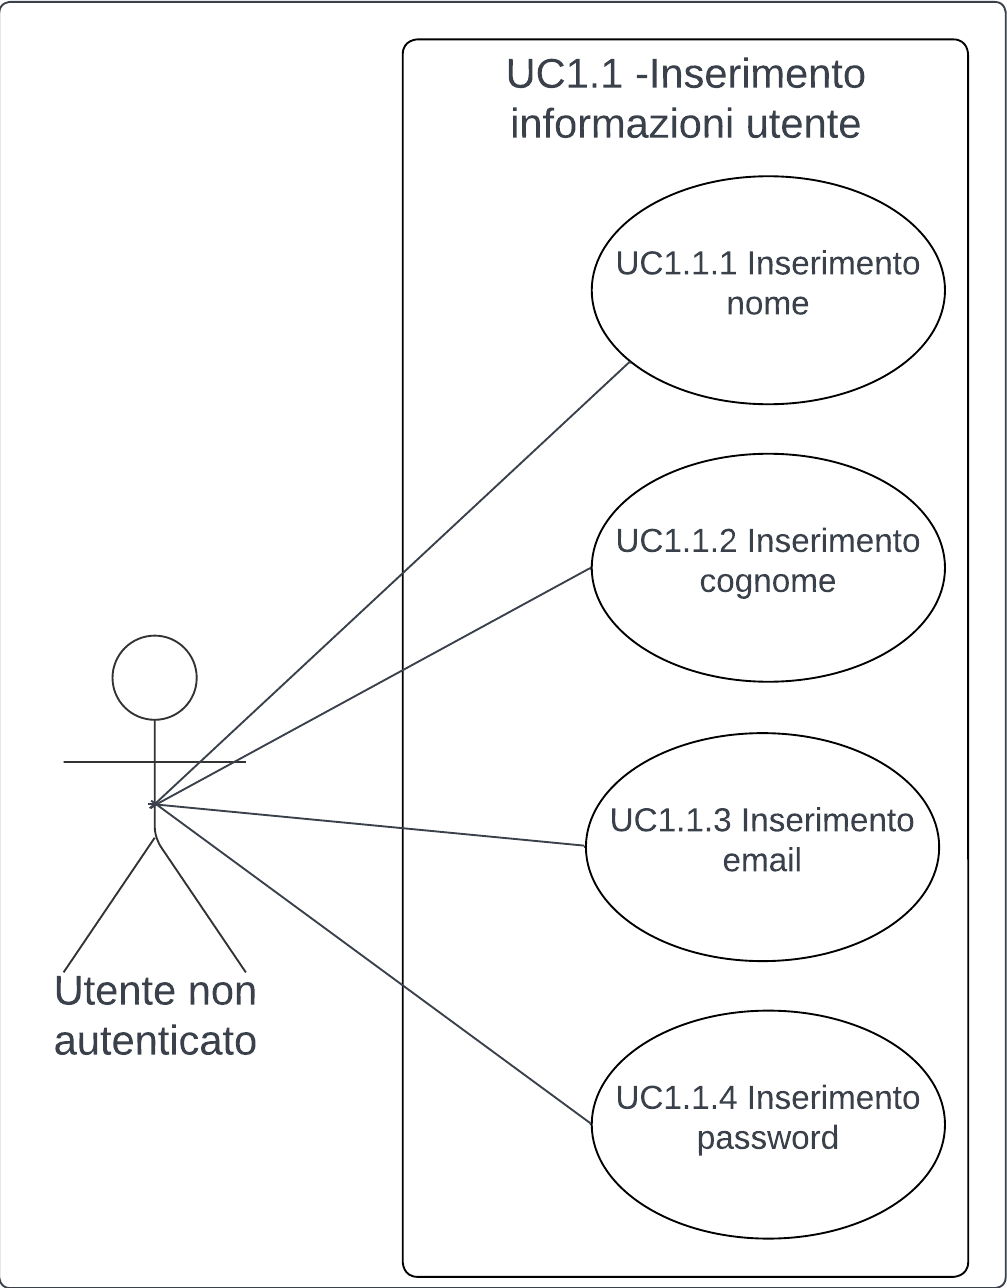
\includegraphics[width=0.4\linewidth]{ucd/UCD1.1.png}
\caption{Registrazione come utente base}
\end{figure}
\textbf{Attori}:
\begin{itemize}
    \item Utente non autenticato.
\end{itemize}
\textbf{Precondizioni}:
\begin{itemize}
    \item L'utente non ha ancora effettuato l'accesso
\end{itemize}
\textbf{Postcondizioni}:
\begin{itemize}
    \item L'utente ha inserito delle credenziali valide
\end{itemize}
\textbf{Scenario principale}:
\begin{enumerate}
    \item l'utente inserisce le sue informazioni:
    \begin{itemize}
        \item nome (\nameref{usecase:1_1_1})
        \item cognome (\nameref{usecase:1_1_2})
        \item email (\nameref{usecase:1_1_3})
        \item password (\nameref{usecase:1_1_4})
    \end{itemize}
\end{enumerate}

\subsubsection{UC1.1.1 - Inserimento nome}\label{usecase:1_1_1}
\textbf{Attori}:
\begin{itemize}
    \item Utente non autenticato.
\end{itemize}
\textbf{Precondizioni}:
\begin{itemize}
    \item L'utente non ha ancora effettuato l'accesso
\end{itemize}
\textbf{Postcondizioni}:
\begin{itemize}
    \item L'utente ha inserito un nome valido all'interno del $\textit{sistema}_G$.
\end{itemize}
\textbf{Scenario principale}:
\begin{enumerate}
    \item l'utente inserisce un nome valido.
\end{enumerate}
\textbf{Scenari secondari}:

\begin{enumerate}
    \item inserimento nome errato:
    \begin{enumerate}
        \item L'utente lascia il nome vuoto;
        \item L'utente usa solo spazi (" ");
        \item L'utente usa caratteri speciali;
        \item L'utente usa caratteri numerici;
    \end{enumerate}

\end{enumerate}


\subsubsection{UC1.1.2 - Inserimento cognome}\label{usecase:1_1_2}
\textbf{Attori}:
\begin{itemize}
    \item Utente non autenticato.
\end{itemize}
\textbf{Precondizioni}:
\begin{itemize}
    \item L'utente non ha ancora effettuato l'accesso
\end{itemize}
\textbf{Postcondizioni}:
\begin{itemize}
    \item L'utente ha inserito un cognome valido all'interno del $\textit{sistema}_G$.
\end{itemize}
\textbf{Scenario principale}:
\begin{enumerate}
    \item l'utente inserisce un cognome valido.
\end{enumerate}
\textbf{Scenari secondari}:

\begin{enumerate}
    \item inserimento cognome errato:
    \begin{enumerate}
        \item L'utente lascia il nome vuoto;
        \item L'utente usa solo spazi (" ");
        \item L'utente usa caratteri speciali;
        \item L'utente usa caratteri numerici;
    \end{enumerate}    
\end{enumerate}

\subsubsection{UC1.1.3 - Inserimento email}\label{usecase:1_1_3}
\textbf{Attori}:
\begin{itemize}
    \item Utente non autenticato.
\end{itemize}
\textbf{Precondizioni}:
\begin{itemize}
    \item L'utente non ha ancora effettuato l'accesso
\end{itemize}
\textbf{Postcondizioni}:
\begin{itemize}
    \item L'utente ha inserito un'email valida all'interno del $\textit{sistema}_G$.
\end{itemize}
\textbf{Scenario principale}:
\begin{enumerate}
    \item l'utente inserisce un indirizzo email valido.
\end{enumerate}
\textbf{Scenari secondari}:

\begin{enumerate}
    \item inserimento di un indirizzo email errato:
    \begin{enumerate}
            \item L'utente lascia il campo email vuoto;
            \item L'utente non inserisce una email nel formato: xxxxx@yyy.zz;
            \item L'utente inserisce una email già registrata;
        \end{enumerate} 
\end{enumerate}

\subsubsection{UC1.1.4 - Inserimento password}\label{usecase:1_1_4}
\textbf{Attori}:
\begin{itemize}
    \item Utente non autenticato.
\end{itemize}
\textbf{Precondizioni}:
\begin{itemize}
    \item L'utente non ha ancora effettuato l'accesso
\end{itemize}
\textbf{Postcondizioni}:
\begin{itemize}
    \item L'utente ha inserito una password valida all'interno del $\textit{sistema}_G$.
\end{itemize}
\textbf{Scenario principale}:
\begin{enumerate}
    \item l'utente inserisce una password valida.
\end{enumerate}
\textbf{Scenari secondari}:

\begin{enumerate}
    \item inserimento di una password errata:
    \begin{enumerate}
            \item L'utente lascia il campo password vuoto;
            \item L'utente inserisce una password troppo corta (minore di 6 caratteri);
            \item L'utente inserisce una password troppo lunga (maggiore di 24 caratteri);
            \item L'utente inserisce una password senza caratteri minuscoli;
            \item L'utente inserisce una password senza caratteri maiuscoli;
            \item L'utente inserisce una password senza caratteri numerici;
            \item L'utente inserisce una password senza caratteri speciali;
        \end{enumerate} 
\end{enumerate}